\section{Methods}

\subsection{Video Acquisition and Preprocessing}
Behavioral data were obtained from video recordings in which a single camera captured four mazes simultaneously. Each recording was therefore structured as a single video file containing the activity of animals in four spatially separated arenas. The videos can be found at \href{https://doi.org/10.7910/DVN/WHH7W2}{Harvard Dataverse}. To enable individual analysis of each maze, videos were automatically split into four quadrants using a custom Python script \href{https://github.com/atanugiri/GhrelinBehaviorQuantification/blob/main/Python_scripts/Utility_functions/split_videos_by_quadrants.py}{\path{split_videos_by_quadrants.py}}.
Each split video was stored and processed independently in subsequent steps [Link to data deposit]. The split videos can be found at \href{https://doi.org/10.7910/DVN/WHH7W2}{Harvard Dataverse}.
\subsection{Pose Estimation with DeepLabCut}
Pose estimation was performed using \textbf{DeepLabCut (v3.0.0rc9)} [Mathis et al., 2018], running with \textbf{PyTorch v2.7.1} and CUDA acceleration on the laboratory workstation, equipped with an NVIDIA T100 GPU. Training was carried out entirely on this GPU system. After model training and generation of pose estimation output, all downstream analyses (feature extraction, statistical analysis) were conducted on a local Apple Silicon laptop. A DeepLabCut project was first initialized with representative videos. Following project creation, additional recordings were incorporated using the command:
\begin{lstlisting}[language=Python]
deeplabcut.add_new_videos(config_path, new_videos, copy_videos=True, extract_frames=False)
\end{lstlisting}
For frame extraction, we sampled five frames per video using automatic uniform sampling. Each frame was cropped manually to retain only the maze region, thereby excluding irrelevant portions of the field of view:
\begin{lstlisting}[language=Python]
deeplabcut.extract_frames(
    config_path, mode='automatic',
    algo='uniform',
    crop='GUI',
    userfeedback=True
)
\end{lstlisting}
The extracted frames were then labeled interactively using:
\begin{lstlisting}[language=Python]
deeplabcut.label_frames(config_path)
\end{lstlisting}
This invoked the \textbf{napari-DeepLabCut GUI}, which allowed manual annotation of predefined body parts specified in the configuration file (Head, Neck, Midback, Lowerback, Tailbase, and four maze corners). Labels were visually verified with:
\begin{lstlisting}[language=Python]
deeplabcut.check_labels(config_path)
\end{lstlisting}
\begin{figure}[htbp]
    \centering
    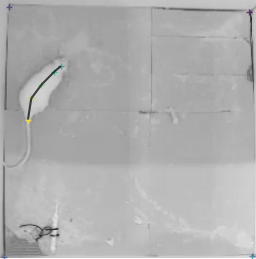
\includegraphics[width=0.8\textwidth]{Figures/label_frames_ex.png}
    \caption{Example of labeled frame.}
    \label{fig:myfigure}
\end{figure}

before generating the training dataset with:
\begin{lstlisting}[language=Python]
deeplabcut.create_training_dataset(config_path)
\end{lstlisting}
Network training was performed with the following settings:
\begin{lstlisting}[language=Python]
deeplabcut.train_network(
    config_path,
    shuffle=1,
    trainingsetindex=0,
    device="cuda:0",
    max_snapshots_to_keep=5,
    displayiters=100,
    save_epochs=5,
    epochs=200,
)
\end{lstlisting}
A ResNet-50 backbone was used, and training proceeded for 200 epochs, with snapshots saved at 5-epoch intervals. 
After training, network accuracy was assessed with:
\begin{lstlisting}[language=Python]
deeplabcut.evaluate_network(config_path, Shuffles=[3], plotting=True)
\end{lstlisting}
Both quantitative error metrics and diagnostic plots were inspected, comparing manual labels against predicted points across training and test frames. Once satisfactory accuracy was achieved, the trained network was applied to all videos using:
\begin{lstlisting}[language=Python]
deeplabcut.analyze_videos(
    config_path,
    videos=videolist,
    shuffle=1,
    gputouse="cuda:0",
    save_as_csv=True
)
\end{lstlisting}
The resulting trajectory files ($x, y, likelihood$ per body part and frame) were further refined using the median filter implementation provided by DeepLabCut:
\begin{lstlisting}[language=Python]
deeplabcut.filterpredictions(
    config_path,
    videolist,
    shuffle=1,
    filtertype='median',
    p_bound=0.05
)
\end{lstlisting}
Filtered CSV files were then used as the input for all downstream feature extraction analyses.


\subsection*{Feature Extraction}
\subsubsection{Trajectory curvature: extraction, aggregation, and statistics}

\paragraph{Project structure and implementation.}
All analyses were run from the project root \path{/Users/atanugiri/Downloads/GhrelinBehaviorQuantification}, which contains two primary directories: \path{DLC-Jupyter-Notebooks/} and \path{Python_scripts/}. The curvature feature was implemented in \href{https://github.com/atanugiri/GhrelinBehaviorQuantification/blob/main/Python_scripts/Feature_functions/trajectory_curvature.py}{\path{trajectory_curvature.py}} and executed from the notebook \href{https://github.com/atanugiri/GhrelinBehaviorQuantification/blob/main/DLC-Jupyter-Notebooks/37_data_analysis_curvature.ipynb}{\path{37_data_analysis_curvature.ipynb}}. Source code will be made available at: \href{https://github.com/atanugiri/GhrelinBehaviorQuantification}{\path{https://github.com/atanugiri/GhrelinBehaviorQuantification}}.

\paragraph{Input data and normalization.}
For each trial, pose trajectories (DeepLabCut outputs) were read from a PostgreSQL database table (\path{dlc_table}). Per-trial frame rate (\path{frame_rate}) was retrieved via SQL and used for all time derivatives. Body-part coordinates were obtained with \href{https://github.com/atanugiri/GhrelinBehaviorQuantification/blob/main/Python_scripts/Data_analysis/normalized_bodypart.py}{\path{get_normalized_bodypart(trial_id, conn, bodypart, normalize=True, interpolate=True)}}, which returns temporally interpolated and spatially min–max normalized coordinates in a fixed, unit-like arena space. Unless otherwise noted, curvature was computed for the \path{Midback} body part (\path{bodypart = 'Midback'}).

\paragraph{Optional time windowing and smoothing.}
Analyses can be restricted to the first $T$ seconds with a \path{time_limit} argument (default: use the full trajectory). When smoothing is enabled, $x(t)$ and $y(t)$ are each convolved with a moving-average (boxcar) filter using \path{scipy.ndimage.uniform_filter1d}. In the notebook runs shown here we used a symmetric window of \path{window_size = 23} samples (odd length enforced internally); smoothing was applied before derivative estimation.

\paragraph{Curvature computation.}
Let $x(t)$ and $y(t)$ be the (optionally smoothed) coordinates, and $\Delta t = 1/\texttt{frame\_rate}$. First and second time derivatives were computed via central differences (\path{numpy.gradient}):
\[
\dot{x}=\frac{dx}{dt},\quad \dot{y}=\frac{dy}{dt},\quad
\ddot{x}=\frac{d^2x}{dt^2},\quad \ddot{y}=\frac{d^2y}{dt^2}.
\]
Per-frame curvature was then defined as
\[
\kappa(t) \;=\; \frac{\left| \dot{x}(t)\,\ddot{y}(t)\;-\;\dot{y}(t)\,\ddot{x}(t) \right|}
{\left( \dot{x}(t)^2 + \dot{y}(t)^2 \right)^{3/2}} \, .
\]
to avoid unstable values at near-zero speeds, frames with speed $v(t)=\sqrt{\dot{x}^2+\dot{y}^2}$ below a threshold were set to $\kappa(t)=0$. We used \texttt{speed\_thresh = 1e-2} (normalized-units/s) unless stated otherwise. The per-trial summary statistic was the mean of all finite $\kappa(t)$ values:
\[
\overline{\kappa} \;=\; \frac{1}{N_\text{valid}}\sum_{t \in \mathcal{V}} \kappa(t),
\]
where $\mathcal{V}$ indexes frames with finite curvature.

\paragraph{Batch processing and grouping.}
For group analyses, we used \path{batch_trajectory_curvature(conn, trial_ids, ...)}, which calls the per-trial routine and returns a table with columns \path{{id, mean_curvature}}. In the notebook we defined trial-ID lists for experimental groups (e.g., \path{Saline}, \path{Ghrelin}, \path{Inhibitory}, \path{Excitatory}), computed \path{mean_curvature} for each trial with \path{window_size = 23}, and concatenated results into a single DataFrame with a \path{group} column.

\paragraph{Statistical testing and visualization.}
Group summaries were visualized with bars (mean~$\pm$~SEM) using a custom plotting utility \href{https://github.com/atanugiri/GhrelinBehaviorQuantification/blob/main/Python_scripts/Data_analysis/plot_groupwise_bar.py}{(\path{plot_groupwise_bar})}. For pairwise comparisons we report both a nonparametric Wilcoxon rank-sum test and a two-sample $t$-test (SciPy \path{ranksums} and \path{ttest_ind}).

\paragraph{Key hyperparameters.}
Unless otherwise noted, we used: \texttt{bodypart = 'Midback'}, \texttt{smooth = True}, \texttt{window = 23} samples, \texttt{speed\_thresh = 1e-2} normalized-units/s, and \texttt{time\_limit = None} (full trial). Per-trial frame rate was read from the database and validated to be $>0$.

All computations were performed in Python (NumPy, SciPy, pandas, Matplotlib) in JupyterLab; code paths and modules are version-controlled within the project directories listed above.


\subsubsection{Velocity (average speed per minute)}

\paragraph{Implementation.}
Velocity was computed with two modules: \href{https://github.com/atanugiri/GhrelinBehaviorQuantification/blob/main/Python_scripts/Feature_functions/motion_features.py}{\path{motion_features.py}} and \href{https://github.com/atanugiri/GhrelinBehaviorQuantification/blob/main/Python_scripts/Feature_functions/motion_features_per_minute.py}{\path{motion_features_per_minute.py}}, and analyzed in the notebook \href{https://github.com/atanugiri/GhrelinBehaviorQuantification/blob/main/DLC-Jupyter-Notebooks/31_data_analysis_distance.ipynb}{\path{31_data_analysis_distance.ipynb}}. Data source, interpolation, and normalization follow the same procedure described in the curvature section.

\paragraph{Per-frame displacement and speed.}
Let $(x_k, y_k)$ denote the (normalized) body-part coordinates at time $t_k = k/\mathrm{frame\_rate}$. We first compute frame-to-frame displacement
\[
d_k \;=\; \sqrt{(x_{k+1}-x_k)^2 + (y_{k+1}-y_k)^2},
\]
and per-frame speed
\[
v_k \;=\; \frac{d_k}{t_{k+1}-t_k} \;=\; \mathrm{frame\_rate}\cdot d_k \quad \text{(for uniform sampling)}.
\]
These arrays are produced by \path{compute_motion_features(...)} together with acceleration (not used here).

\paragraph{Average speed per minute.}
Our scalar velocity metric for each trial is the time-averaged speed expressed in units/min:
\[
v_{\mathrm{per\;min}} \;=\; \frac{\sum_k d_k}{t_{N}-t_0}\times 60,
\]
which is equivalent to $\big(\overline{v}\big)\times 60$. This is returned by \path{compute_motion_features_per_minute(...)}. Trials shorter than a minimum duration (default \path{min_duration_s = 5.0}) yield \path{NaN}.

\paragraph{Key hyperparameters.}
Unless noted otherwise, velocity was computed for the \path{Head} body part (\path{bodypart = 'Head'}), with no temporal smoothing (\path{smooth = False}, \path{window = 5}) and no time cap (\path{time_limit = None}). Frame rate was read per trial from the database.

\paragraph{Batching, grouping, and statistics.}
For each group (e.g., \path{Saline}, \path{Ghrelin}, \path{Inhibitory}, \path{Excitatory}), we computed one value of $v_{\mathrm{per\;min}}$ per trial using \path{batch_compute_motion_features_per_minute(...)} and combined results into a single DataFrame with columns \path{{trial_id, velocity_per_min, group}}. Plots and pairwise statistical tests were generated with \path{plot_groupwise_bar} using the same procedures described for curvature (Wilcoxon rank-sum and Welch’s two-sample $t$-test; see Statistical testing in the curvature section).


\subsubsection{Head–body angle (radians)}

\paragraph{Implementation.}
Angle features were computed with \href{https://github.com/atanugiri/GhrelinBehaviorQuantification/blob/main/Python_scripts/Feature_functions/angle_features.py}{\path{angle_features.py}} and analyzed in \href{https://github.com/atanugiri/GhrelinBehaviorQuantification/blob/main/DLC-Jupyter-Notebooks/40_data_analysis_angle_features.ipynb}{\path{40_data_analysis_angle_features.ipynb}}. As in the curvature section, trajectories and frame rates were obtained per trial. This module reads the raw DeepLabCut CSV path from the database and loads the required body parts directly from the CSV.

\paragraph{Definition.}
We defined two vectors per frame:
\[
\mathbf{v}_{\text{body}} = \mathbf{h} - \mathbf{t} \quad \text{(Tailbase $\to$ Head)}, 
\qquad
\mathbf{v}_{\text{head}} = \mathbf{h} - \mathbf{n} \quad \text{(Neck $\to$ Head)},
\]
where $\mathbf{h}, \mathbf{n}, \mathbf{t}$ are the Head, Neck, and Tailbase coordinates. The \emph{head–body angle} $\theta_{\mathrm{HB}}(t)$ is the signed angle (radians) between these vectors,
\[
\theta_{\mathrm{HB}}(t) \;=\; \operatorname{atan2}\!\big(u_x v_y - u_y v_x,\; \mathbf{u}\!\cdot\!\mathbf{v}\big),
\quad \text{with } \mathbf{u}=\mathbf{v}_{\text{body}},\; \mathbf{v}=\mathbf{v}_{\text{head}}.
\]
By convention, positive values indicate a counterclockwise rotation of the head relative to the body axis; $\theta_{\mathrm{HB}}(t)\in(-\pi,\pi]$ per frame.

\paragraph{Summary metric and statistics.}
For each trial we summarized the head–body angle by its 95th percentile (radians). Group plots and pairwise comparisons followed the curvature section (Wilcoxon rank–sum and Welch’s two-sample $t$-test).






% \paragraph{Body orientation and angular velocity.}
% The global body orientation was $\theta_{\text{body}}(t)=\operatorname{atan2}\!\big(\mathbf{v}_{\text{tail}\to\text{head}}\big)$ (via \path{_angle_of}). We applied phase unwrapping (\path{np.unwrap}) to obtain a continuous $\theta_{\text{body}}$ trace. If \path{smooth_window} is specified, an odd-length moving average is applied to the unwrapped $\theta_{\text{body}}$ prior to differentiation. Angular velocity was then computed by central differences,
% \[
% \omega_{\text{body}}(t)=\frac{d\,\theta_{\text{body}}(t)}{dt}\quad\text{(rad/s)}.
% \]
% For convenience, per-minute values are reported as $\omega_{\text{body}} \times 60$ (rad/min) where indicated.

% \paragraph{Per-trial summaries and primary outcome.}
% For each timeseries we recorded summary statistics \path{mean}, \path{std}, \path{max}, and 95th percentile (\path{p95}). The \emph{primary head–body angle outcome} used in group comparisons was the 95th percentile of the head–body misalignment distribution, \path{head_body_misalignment_p95} (radians), taken directly from $\phi(t)$.%
% \footnote{If a magnitude-only measure is preferred, one can compute the percentile on $|\phi(t)|$; our analyses used the signed distribution’s 95th percentile as implemented.}

% \paragraph{Batching, grouping, and statistics.}
% For each group (e.g., \path{Saline}, \path{Ghrelin}, \path{Inhibitory}, \path{Excitatory}), we ran \path{batch_angle_features(...)} and collected \path{{trial_id, head_body_misalignment_p95}} into a single DataFrame with a \path{group} column. Plots and pairwise tests were produced with \path{plot_groupwise_bar} as described for curvature (Wilcoxon rank-sum and Welch’s two-sample $t$-test).


% \subsection*{Feature Extraction}

% \textbf{Trajectory curvature.}
% Curvature of locomotor trajectories was computed from body part coordinates obtained with DeepLabCut. For each trial, we used the midline marker (Midback) as the reference point for tracking the animal’s path. The x--y coordinates were first smoothed with a moving average filter to reduce frame-to-frame noise. 
% % Instantaneous curvature was calculated as the rate of change of the trajectory’s tangent angle with respect to arc length.
% Trials with frame-wise velocity below a minimum threshold were excluded from curvature calculation to avoid artifacts from immobility. For each trial, we summarized curvature using both the mean value across the entire trajectory and additional statistics (e.g., maximum and variability), which were used for downstream analyses. Code implementation is available at \href{https://github.com/atanugiri/GhrelinBehaviorQuantification/blob/main/Python_scripts/Feature_functions/trajectory_curvature.py}{\path{trajectory_curvature.py}}.

% \textbf{Velocity.}  
% Velocity was derived from the inter-frame displacement of the Midback marker normalized by the frame rate of the video. Specifically, instantaneous speed was computed as the Euclidean distance between consecutive positions divided by the frame interval. To account for potential jitter, the velocity signal was smoothed using a centered moving window. Trial-level features included mean velocity, peak velocity, and velocity profiles segmented over time bins to capture within-trial dynamics.  
% Code implementation is available at \href{https://github.com/atanugiri/GhrelinBehaviorQuantification/blob/main/Python_scripts/Feature_functions/motion_features.py}{\path{motion_features.py}}.

% \textbf{Head--body angle.}  
% The head--body angle was quantified as the angle formed between the head vector (Head $\rightarrow$ Neck) and the longitudinal body axis (Midback $\rightarrow$ Lowerback). At each frame, we computed the dot product between the two normalized vectors to obtain the angular deviation in degrees. This measure reflects head orientation relative to the body axis and has been used as a proxy for exploratory head scanning or directional misalignment. For each trial, we extracted the distribution of angles and reported summary measures such as mean, maximum, and upper percentiles.  
% \href{https://github.com/atanugiri/GhrelinBehaviorQuantification/blob/main/Python_scripts/Feature_functions/angle_features.py}{\path{angle_features.py}}.

% % Exploration

% \subsection*{Statistical treatment}
% All feature values were aggregated at the trial level. Trials containing missing or low-confidence DeepLabCut detections (likelihood $<$ threshold) were excluded from analysis. 